\section{Évaluation du projet}
\subsection{Validation du logiciel} %validation des fonctionnalités du logiciel ..?
\subsubsection{Visualisation}
parler de fps, de maniabilité de la scène 3D, de la GUI

\subsubsection{Communication réseau}
parler de latence, de l'établissement de la connection (qui foire de temps en temps, essayer de faire peut être plusiuers tests pour établir une moyenne), de la perte de paquets éventuelle ..?

\subsubsection{Simulation}
parler des aspects simulation, la proximité à la réalité (comparer le modèle théorique au modèle réelle si possible, mais les tests réelles avec les metabots risquent d'être compromis ...)

\subsubsection{Bilan validation}
reprendre sous forme de tableau ce qui a été cité précédemment ?

\subsection{Gestion du projet: calendrier et difficultés}

Dans cette partie, nous verrons la gestion du projet par rapport au calendrier que nous nous étions fixé. Puis nous verrons les difficultés que nous avons rencontrées. Le calendrier prévu était celui représenté sur la figure suivante \ref{cal}:

\begin{figure}[H]
  \begin{center}
  	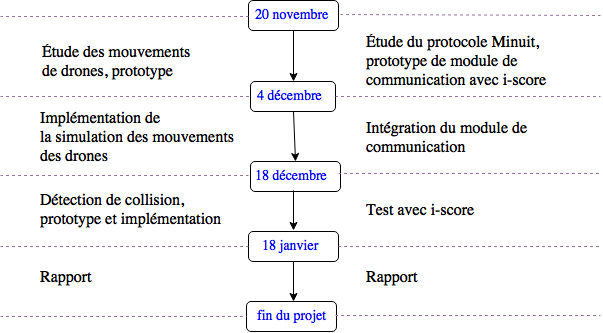
\includegraphics[scale=0.7]{imgs/calendrier.png}
  	\caption{Calendrier initial}
  	\label{cal}
  \end{center}
\end{figure}

Finalement, ce calendrier ne représente pas vraiment ce qui a été réalisé. D'une part, la partie de simulation des mouvements des drones a été abandonnée car le projet s'est focalisé sur la mise en place des métabots en premier. D'autre part, la partie communication ne s'est pas déroulée comme prévu. L'intégration de la communication avec i-score dans simulationRainOfMusic nous a pris du temps au niveau de l'intégration de l'API d'OSSIA. Ensuite, la communication avec i-score se fait assez facilement. Le problème qui est apparu ensuite est la synchronisation entre l'interface de simulationRainOfMusic et i-score, cf LOOP. 

loop: gui param i-score, pas moyen de différencier si la valeur est mise à jour depuis i-score ou à la main sur un slider.
